\chapter{Results}\label{sec:res}
\section{BabelStream}\label{sec:res-babel}
Figures~\ref{fig:babel-dot},~\ref{fig:babel-add} and~\ref{fig:babel-triad} all show that Rust and C++ have similar performance but that at higher thread counts, there is a great deal of difference between the threaded performance of both implementations. In each figure, the amount of megabytes refers to how large a subsection of the total data the threads are assigned to work on. If not stated, the library's own chunking strategy was used.

For example, both Rust and C++ have very similar memory bandwidths in the Dot product's serial execution. Rust's bandwidth here is 11.5 GB/s and C++'s is 11.6 GB/s, giving a difference of just 1\%.
However, this difference later widens at 32 threads to 65\% with Rust at 87.3 GB/s and C++ at 135.1 GB/s.

\begin{figure}[h]
\centering
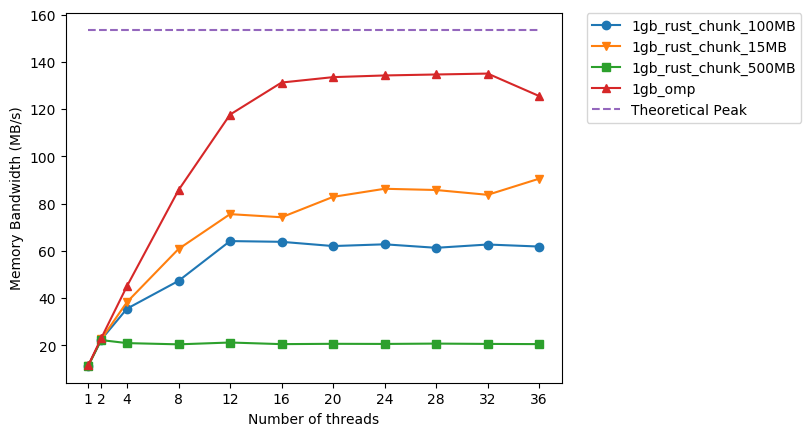
\includegraphics[width=.9\linewidth]{figs/babel/Dot.png}
\caption[BabelStream --- Dot]{BabelStream --- Dot product bandwidth against number of threads}\label{fig:babel-dot}
\end{figure}

The performance difference is similar for both the add and triad benchmarks, at 66\%, implying a consistent negative performance factor for Rust and Rayon. The results for add and triad are shown in figure~\ref{fig:babel-add} and~\ref{fig:babel-triad}.
It is interesting that the dot product is able to attain a higher level of memory bandwidth. It is most likely because the dot product is only reading from the arrays, not writing to them, which lessens the amount of cache invalidation.

Notably the rate of improvement in memory bandwidth decreases sharpely between 16 and 20 threads. This decrease is probably due to each processor only having 18 cores. Requiring data to pass across the CC-NUMA regions adds a significant communication overhead, which slows the rate of increase in memory bandwidth.
\begin{figure}[h]
\centering
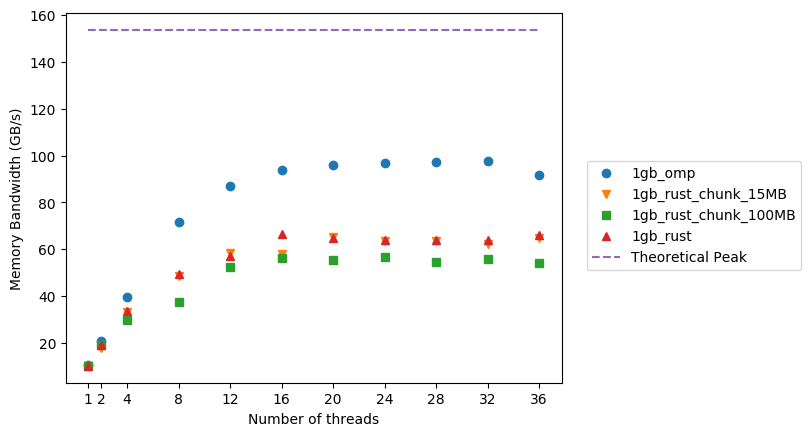
\includegraphics[width=.9\linewidth]{figs/babel/Add.png}
\caption[BabelStream --- Add]{BabelStream --- Add bandwidth against number of threads}\label{fig:babel-add}
\end{figure}

This increasing difference suggests that an examination of assembly code would not be beneficial in this circumstance. Instead, it seemed like the threading implementation was so different that it was what was causing the problem, which is much easier to understand in its high level expression. I decided to investigate the thread scheduling implementation.

\begin{figure}[h]
\centering
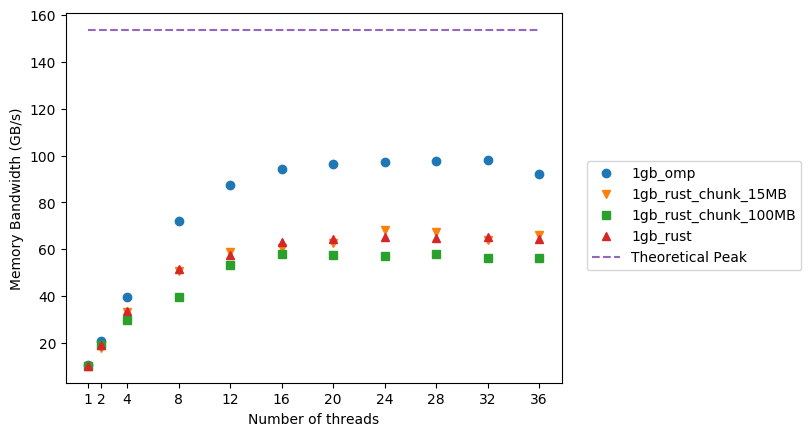
\includegraphics[width=.9\linewidth]{figs/babel/Triad.png}
\caption[BabelStream --- Triad]{BabelStream --- Triad bandwidth against number of threads}\label{fig:babel-triad}
\end{figure}

There was also the possibility that Rayon's algorithm for loading data for threads was more costly to performance than OpenMP's. However, this would likely need to be confirmed at the level of assembly instructions, which can be difficult to parse. Therefore, it seemed like a much better strategy to look at how thread scheduling in Rayon works  and also look out for hints of context switching costs.

Consulting the documentation reveals that Rayon's \texttt{par\_iter()} construct reveals that the parallel iterator API is a wrapper around Rayon's \texttt{join()} method~\cite{smallCult}. In the source code for \texttt{join()}, it is stated that the underlying implementation of join in Rayon is different to the common conception of it. 
`The underlying technique is called ``work stealing'': the
Rayon run time uses a fixed pool of worker threads and attempts to only execute code in parallel when there are idle CPUs to handle it'~\cite{joinSrc}.

Work stealing is an established parallel technique, in which threads work on chunks of computation, and when they have finished their chunk, they steal chunks of computation from other threads~\cite{blumofe1999}. This reactive method of scheduling is very good at dealing with unanticipated work loads, when it is not known where the bulk of the computation will take place.

A dynamic schedule will often do poorly compared to a static schedule, when the workload is evenly distributed amongst threads. The default OpenMP parallel for schedule is a static one, which evenly splits the work between threads~\cite{OpenMPSpec5}. The effect of this schedule is that data is more likely to work on data which it has initialised, which is likely to be within the same CC-NUMA region, and therefore quicker to access. In comparison, the work which threads will do in a work stealing schedule is non deterministic, and may require to be fetched from further away, at greater cost.

Although the results for BabelStream do show that in this particular circumstance, OpenMP does have higher performance, it does not necessarily follow that the static schedule will always be best for HPC\@.

\section{Sparse Matrix Vector Multiplication}\label{sec:res-sparse}

The Roofline model in figure~\ref{fig:roofline} shows there was very little difference in performance between the two implementations of the kernel.

Using \texttt{perf} showed that only the C version of SpMV used instructions with the code \texttt{r5310c7}, which is used for packed 256 bit instructions. In this case, it was used to add four doubles together when performing the matrix vector multiplication and storing the result in \texttt{temp}\footnote{line 290 of sparse.c}. Both implementations used 64 bit and 128 bit instructions. 

\begin{figure}[h]
\centering
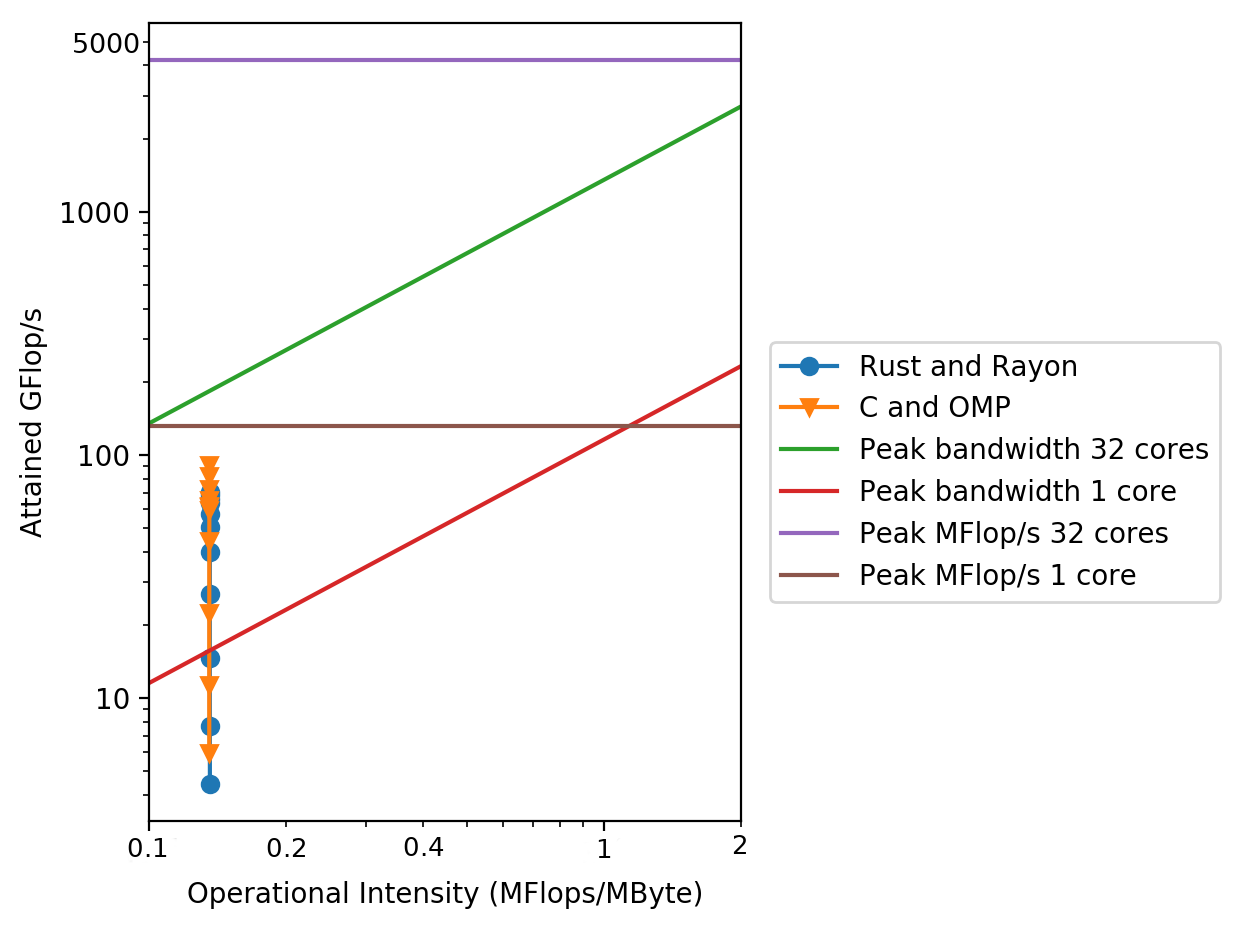
\includegraphics[width=.75\linewidth]{figs/sparse/roofline.png}
\caption[SpMV --- Roofline model]{SpMV --- Roofline model shows similar performance for both implementations of the kernel. For clarity, only every other datum from each data set has been used. Thread count ranged between 1 and 36 threads, with lower thread counts attaining lower GFlop/s.}\label{fig:roofline}
\end{figure}

Figure~\ref{fig:roofline} compares the execution of both implementations of the SpMV Kernel using the Roofline model. Operational intensity shows itself to be very low, at around 0.13 Flops/Byte. This is equivalent to 1.04 Flops per double.\todo{include rupe's thing!}
Although this is a low amount of Flops per double, SpMV is known to not have a high operational intensity~\cite{SparseArith}. Roughly one Flop per double is to be expected from the algorithm used, and the sparsity of the matrix, as each double in the SpMV matrix is used only once in each iteration. I have also counted the \texttt{col\_index} array in generating this Roofline model, because although it does not contain floating point numbers, it is needed to perform any Flops.
It is remarkable that the performance of both implementations is so similar. Whilst C has slightly higher performance, and Rust marginally better operational intensity, both implementations are clearly memory bandwidth bound. 

Figure~\ref{fig:sparse-time} helps to clarify further the difference in performance between  the two implementations.  Whilst Rust is slower than C at most thread counts, it is never an order of 2 slower.
The Rust implementation is even slightly faster than C implementation at twenty threads. 
\begin{figure}[h]
\centering
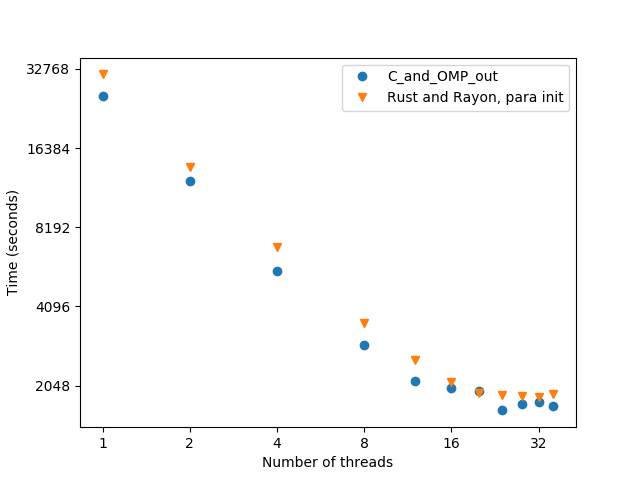
\includegraphics[width=.9\linewidth]{figs/sparse/time.png}
\caption[SpMV --- Time]{SpMV --- Time taken for SpMV to complete against number of threads. A $\log_2 \log_2$ scale has been used here to make the difference in performance clearer.}\label{fig:sparse-time}
\end{figure}

Compared to the results from BabelStream, Rust performs a lot better. This could be because the work stealing schedule for Rayon is better suited to SpMV irregular work distribution, whilst OpenMP's usage of static scheduling is sub optimal. However, it is impossible to conclusively make such a statement without further work, which is outlined in greater detail in Section~\ref{sec:furth}.


\section{K-means clustering}\label{sec:res-kmeans}

As in the SpMV results, the time taken for the K-means clustering by both implementations does not differ greatly. Figure~\ref{fig:kmeans-time} shows that on three occasions, Rust and Rayon was faster than C and OpenMP\@. It is noteworthy that two of these occasions occur at the boundaries of the experiment.

At one thread, Rust carries out the E-step faster than C does. This result is interesting, because it implies that if Rust could use an threading API that had the same schedule and overheads as OpenMP, then it could theoretically be faster than it. However, the difficulty of writing a threading API in Rust which is as optimised as OpenMP, a standard that's implementations have been continually optimised for more than two decades, should not be underestimated.

\begin{figure}[h]
\centering
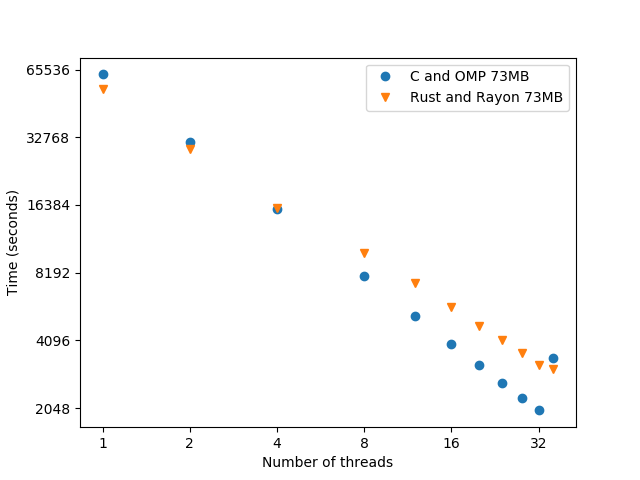
\includegraphics[width=.9\linewidth]{figs/kmeans/time.png}
\caption[K-means --- Time]{K-means --- Time taken for E-step to complete against number of threads, on a $\log_2 \log_2$ scale.}\label{fig:kmeans-time}
\end{figure}

At 36 threads, Rust is marginally faster than C. This result is interesting not because of Rust's speedup, but because of C's slowdown. The time taken for the C implementation to complete its E-step almost doubles between 32 and 36 threads, whereas the amount of time the Rust implementation takes slightly decreases. This is a similar pattern to the results shown by BabelStream, and is most noticeable in figure~\ref{fig:babel-dot}.
In all the BabelStream figures, the performance of the kernel's C implementation decreases between 34 and 36 threads, whilst Rust improves slightly.

I hypothesise that this difference in performance at 36 threads occurs because at this point, all of the processor's cores are being used. At this stage, one of the threads must share a core with operating system threads. This sharing results in one of the threads taking longer to complete its section of work, because it must share its resource with the operating system. OpenMP's default static schedule does not perform well in this circumstance, as each thread must do an equal amount of work, no matter how long individual threads take to do their portion of work.
This results in other threads waiting for the 36$^{th}$ thread, which is sharing a core with the operating system, to finish its work.

In comparison, Rayon's work stealing schedule allows threads which finish early to take work from slower threads. Therefore, instead of finished threads waiting for the slower 36$^{th}$ thread, they can take work from it, and not need to wait. To confirm this hypothesis, I would either need to implement a work stealing schedule for OpenMP, or a static schedule for Rust, and compare the results.

\section{Questionnaire}\label{sec:res-q}
Figure~\ref{fig:questions} presents the collected data from the questionnaire. Each small dot represents one answer, and a larger dot represents two. Eleven responses were collected in total. None of the participants claimed any level of knowledge of Rust.
These results show no correlation between competency and score. This suggests that it is difficult to predict how easy a HPC programmer will understand Rust. 

\begin{figure}[h]
\centering
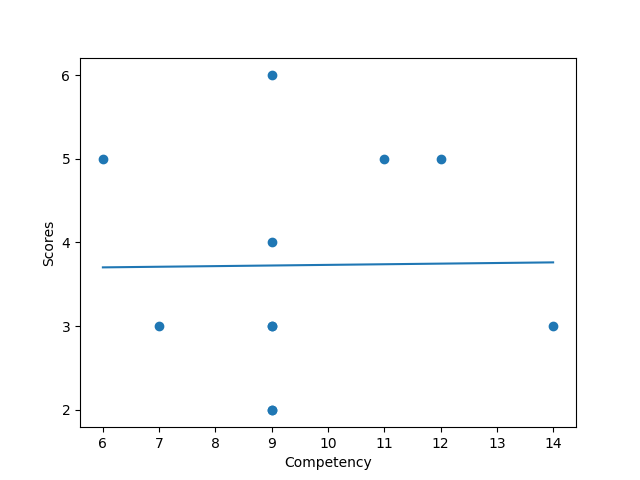
\includegraphics[width=.8\linewidth]{figs/questions/scatter.png}
\caption[Questionnaire Results]{Questionnaire --- Score against Competency. Larger dots indicate greater frequency}\label{fig:questions}
\end{figure}

However, as these such little data was collected in this circumstance, it would be unreasonable to claim that this study contains any decisive information. The study would need to be carried out a second time, with a much larger group of participants.

Interesting highlights from the data show that knowledge of programming languages often thought similar to Rust, like Haskell, did not necessarily predict if the participant would score highly on their Rust questions. One particular participant rated their level of competency in Haskell as basic. The participant did answer Q4 of the questionnaire correctly, which deals with optional values and pattern matching, which are common concepts within Haskell. However, the participant was only able to answer another two of the seven questions correctly, and therefore did not do any better than most of the participants. Questions that the participant answered incorrectly included when programs should not compile due ownership and mutability violations, and the result of chaining method calls.

This result, and the participant who scored themselves a fourteen in competency and yet received a score of three, suggest that Rust's range of programming paradigms require learning, and cannot simply be assumed to be known from other languages.
